% Im Juni 2000 stellte das Unternehmen Microsoft das \ac{dotnet} vor.
% Kurz darauf wurde von Miguel de Icaza das sogenannte Mono-Projekt als Open-Source gestartet, welches eine Linux-Version des \ac{dotnet} darstellen soll.
% Am 16. Mai 2011 kündigt Miguel de Icaza an, dass das Mono-Projekt vom Unternehmen Xamarin weiterentwickelt wird, wobei einige wichtige Mitglieder des Mono-Entwickler-Teams weiterhin daran beteiligt sind.

% Das Unternehmen Xamarin wurde mit der Absicht gegründet, Software auf mobile Geräte zu vertreiben. 
\label{ch:prog-doc}
\section{Übersicht}
Das im Zuge dieser Diplomarbeit entwickelte Software-Projekt basiert auf einer der von Microsoft bereitgestellten Xamarin.Forms-Vorlagen, welche als Teil von Visual Studio bereitgestellt werden.
Es gibt mehrere Auswahlmöglichkeiten, wobei alle Vorlagen bis auf \enquote{Blank} Beispielcode beinhalten.
Da der Beispielcode der anderen Vorlagen für dieses Projekt nicht relevant ist und ohnehin gelöscht werden müsste, wird die \enquote{Blank}-Vorlage verwendet.
Diese Vorlage beinhält nur eine Haupt-Oberflächenseite ohne jeglichen Beispielcode.

Der immer wieder vorkommende Name PiBell ist eine freigeistliche Erfindung. PiBell ist der Projektname, der sich aus \acl{rpi} und \enquote{Bell}, dem englischen Wort für Klingel oder Glocke, zusammensetzt.

Visual Studio organisiert alle Programmteile in einer sogenannten Solution, welche den Projektnamen trägt. In diesem Fall beinhält die Solution \enquote{PiBell} drei Programmteile oder \enquote{Projects}:
\paragraph{PiBell} ist das portable Projekt, auch .NET-Standard-Projekt genannt.
Dieses beinhaltet den ganzen plattformunabhängigen Code, sowie die Definition der UI-Oberfläche mittels XAML-Dateien.
In diesem Projekt befindet sich der größte entwickelte Code-Anteil, da die meisten Funktionen, wie das Abspielen von Videos mit Hilfe der LibVLC-Bindings, plattformunabhängig funktionieren und deswegen geteilt werden können.

\paragraph{PiBell.Android} beinhaltet allen Code, der plattformspezifisch für Android geschrieben wurde.
Unter anderem ist hier enthalten die Android-Implementation des Mikrofon-Auf\-nahme-Services, sowie das Berechtigungs-Management.
Die Mikrofon-Aufnahme erfolgt auf einer sehr hardwarenahen Ebene, was die plattformabhängigkeit erklärt.

\paragraph{PiBell.iOS} beinhaltet wie PiBell.Android den plattformspezifischen Code für die iOS-Platt\-form. Aufgrund mangelnder Entwicklungswerkzeuge wurde dieser Teil nicht großartig behandelt.\par

\begin{figure}[H]
\centering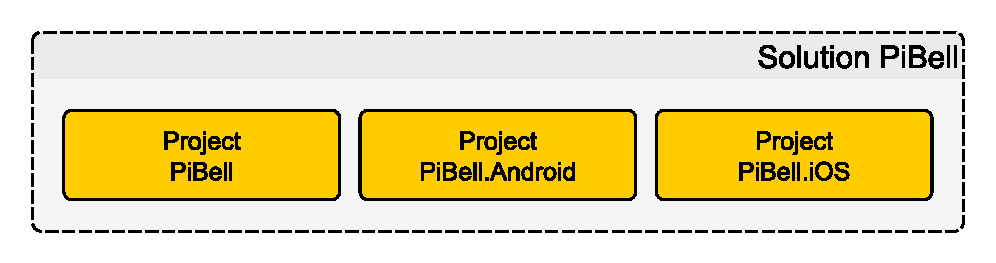
\includegraphics[width=0.9\linewidth]{images/xamarin/struktur.pdf}
\caption{Aufbau der Solution}
\end{figure}

%besteht aus drei teilen
%- portable project/.net standard project
%   plattformunabhängiger teil, oberfläche, ...
%- Android project
    %android-spezifischer teil, berechtigungen, ...
%- iOS project
    %iOS-spezifischer Teil, ...
%project-name PiBell -> erfindung, leitet sich aus raspberry und Türglocke ab
%
\section{Portable Project}
\subsection{App.xaml.cs}
\begin{lstlisting}[firstnumber=17]
public App()
{
    InitializeComponent();
    Core.Initialize();
    MainPage = new MainPage();


    AppCenter.LogLevel = Microsoft.AppCenter.LogLevel.Verbose;
    AppCenter.Start("android=2234efba-9d8c-45ec-bfad-f78aaa6ba632;" +
                    "uwp={Your UWP App secret here};" +
                    "ios={Your iOS App secret here}",
        typeof(Analytics), typeof(Crashes), typeof(Push));
}
\end{lstlisting}
\paragraph{19/20:} Die Funktionen InitializeComponent() und Core.Initialize sind vorgefertigte Funktionen; diese sind zu verwenden um die Applikation und alle benötigten Bibliotheken zu initialisieren.
\paragraph{21:} Die Anweisung MainPage = new MainPage() erzeugt eine neue Oberfläche, mit der der Benutzer mit der App interagiert. Diese Oberfläche erscheint nach dem App-Start am Bildschirm und passt sich automatisch der physikalischen Bildschirmgröße an.
\paragraph{24-28:} Mit AppCenter.LogLevel kann festgelegt werden, welche Log-Nachrichten angezeigt werden. In diesem Fall werden Alle Nachrichten aktiviert.
Anschließend wird das AppCenter SDK mit AppCenter.Start(..) gestartet. Am Ende dieser Anweisung werden alle Module (Analytics, Crashes und Push), die dazu gestartet werden sollen angegeben.

\subsection{MainPage.xaml}
%vlcht. Zu Xamarin im Allgemeinen
In einer XAML-Datei wird das Aussehen der Oberfläche nach dem WYSIWYM-Prinzip beschrieben. Das Format ähnelt sehr einer XML-Datei, in der Hinsicht, dass ein Element mit einer spitzen Klammer (<) beginnt und mit einem Schrägstrich und einer spitzen Klammer (/>) endet. Einige Elemente, wie zum Beispiel Listen oder ein Grid, können sogenannte Kind-Elemente beinhalten.
\begin{lstlisting}[firstnumber=3,language=xml]
<ContentPage xmlns="http://xamarin.com/schemas/2014/forms"
             xmlns:x="http://schemas.microsoft.com/winfx/2009/xaml"
             xmlns:local="clr-namespace:PiBell"
             xmlns:piBell="clr-namespace:PiBell;assembly=PiBell"
             xmlns:shared="clr-namespace:LibVLCSharp.Forms.Shared;assembly=LibVLCSharp.Forms"
             x:Class="PiBell.MainPage"
             Title="Main Page"
             BackgroundColor="#ff1b1b1b">
\end{lstlisting}
\paragraph{3-8:} Am Anfang der XAML-Datei wird der allgemeine Seiten-Typ, gemeinsam mit einigen Quell-Abkürzungen (Namenspräfix für Xamarin-fremde Elemente) definiert. In diesem Fall handelt es sich um eine simple ContentPage mit den Standard-Abkürzungen. Zur Verwendung der LibVLC wurde in Zeile 7 eine zusätzliche Quelle definiert. Die neu hinzugefügte Quelle erlaubt den Zugriff auf Elemente wie die VideoView, welche ein Video als Teil der Oberfläche darstellt.
\paragraph{9:} Mit x:Class wird die Programmklasse angegeben, die den Code der Oberfläche beinhält. In dieser Klasse finden sich alle Event-Handler für jegliche Oberflächenereignisse, wie das drücken eines Buttons.
\paragraph{10:} Das festlegen der Title-Variable ist in diesem Fall optional. Falls eine Master-Detail-Page-Struktur verwendet werden würde, wäre der Titel oben in der Kopfzeile der App zu sehen. Da es sich hier aber um ein Sigle-Page-Layout handelt, ist der Titel nicht zwingend notwendig.
\paragraph{11:} Mit der Variable BackgroundColor wird die Hintergrundfarbe der Oberfläche definiert. Die gewünschte Farbe wird als HEX-Zahl mit dem Format Alpha-Rot-Grün-Blau angegeben. Der Alpha-Wert legt die Durchsichtigkeit der Farbe fest. Es wurde sich für ein dunkles Design entschieden, da dieses in einer wenig beleuchteten Umgebung die Augen besser schont.

\begin{lstlisting}[firstnumber=12,language=xml]
<ContentPage.Content>
    <Grid Margin="10" x:Name="MainGrid">
        <Grid.RowDefinitions>
            <RowDefinition Height=".7*" />
            <RowDefinition Height="3*" />
            <RowDefinition Height="2*" />
        </Grid.RowDefinitions>
        <Grid.ColumnDefinitions>
            <ColumnDefinition Width="*" />
        </Grid.ColumnDefinitions>
\end{lstlisting}
\paragraph{12:} Mit dieser Zeile wird das Element ContentPage.Content geöffnet. Content steht hier für den gesamten Oberflächeninhalt, also alle Schaltflächen und Anzeigen.
\paragraph{13-21:} Als erstes und einziges Kind-Element von ContentPage.Content wird die Komponente Grid gewählt. Diese ermöglicht es, mehrere Kind-Elemente in einer schachbrettartigen Anordnung zu organisieren. Hierfür werden mit Hilfe der Row- und ColumnDefinitions die Höhen und Breiten der einzelnen Zeilen und Spalten festgelegt. Der Stern (*) in der Längenangabe bedeutet relatives Maß bezogen auf die verfügbare Breite bzw. Höhe.
\begin{lstlisting}[firstnumber=23,language=xml]
<Entry x:Name="EditMrl" Text="{Binding Mrl, Mode=TwoWay}" Grid.Row="0" Grid.Column="0" TextColor="White" />

<shared:VideoView x:Name="VideoView" Grid.Column="0" Grid.Row="1" MediaPlayer="{Binding MediaPlayer}"/>
\end{lstlisting}
\paragraph{23:} Hier wird das erste eigenständige Oberflächen-Element erzeugt. Es handelt sich um ein Text-Eingabe-Feld (Entry), mit dem zu Testzwecken die Serveradresse eingegeben werden kann. Dies ist notwendig, da die finale Serveradresse noch nicht bekannt ist und sich diese im Zuge der Entwicklung ständig ändert. Für den späteren Betrieb könnte dieses Problem umgangen werde, indem die aktuelle Server-Adresse per Push-Benachrichtigung mitgeschickt wird. Hier ist auch eine Anwendung des MVVM-Modells erkennbar: es wird mit Hilfe des Binding-Schlüsselwortes der Speicherort des angezeigten Textes festgelegt. Mode=TwoWay beschreibt die Richtung der Synchronisierung der Daten. Egal, ob sich der Wert im Speicher oder der Wert in der Anzeige ändert, wird die jeweils andere Seite aktualisiert. Mit Grid.Row und Grid.Column wird die Position im vorhin definierten Grid gesetzt.
\paragraph{25:} Das zweite Oberflächen-Element, eine VideoView der LibVLC, wird hier erzeugt. Da die Komponente VideoView nicht standardmäßig in Xamarin enthalten ist, wird das am Anfang der Datei definierte Namenspräfix „shared:“ benötigt.

\begin{lstlisting}[firstnumber=36,language=xml]
<ImageButton x:Name="BtConnect" Source="call.png" BackgroundColor="LimeGreen" Grid.Row="0"
             Grid.Column="0" Margin="10"
             Clicked="BtConnect_Clicked"/>
\end{lstlisting}
\paragraph{36:} Ein ImageButton kann im Vergleich zu einem normalen Button als Inhalt ein Bild anzeigen. Die Bildquelle wird mit der „Source“-Property gesetzt. Es gibt mehrere mögliche Bildformate, wobei hier PNG aufgrund von Transparenz-Unterstützung gewählt wurde. Ohne Definition der „BackgroundColor“ würde der ImageButton mit der Default-Farbe grau gefüllt werden.
\paragraph{38:} Mit dem EventHandler „Clicked“ kann die Funktion, die aufgerufen wird wenn der ImageButton gedrückt wird, spezifiziert werden.
\begin{lstlisting}[firstnumber=43,language=xml]
<ImageButton x:Name="BtToggleSpeaker" Source="SpeakerMute.png" BackgroundColor="Transparent"
             Grid.Row="1" Grid.Column="0" Margin="10"
             Clicked="BtToggleSpeaker_Clicked">
    <VisualStateManager.VisualStateGroups>
        <VisualStateGroup x:Name="SpeakerStates">
            <VisualState Name="Mute">
                <VisualState.Setters>
                    <Setter Property="Source"
                            Value="SpeakerMute.png" />
                </VisualState.Setters>
            </VisualState>
            <VisualState Name="Unmute">
                <VisualState.Setters>
                    <Setter Property="Source"
                            Value="SpeakerUnmute.png" />
                </VisualState.Setters>
            </VisualState>
        </VisualStateGroup>
    </VisualStateManager.VisualStateGroups>
</ImageButton>
\end{lstlisting}
\paragraph{47-62:} Mit dem VisualStateManager können für die meisten Oberflächen-Elemente bestimmte Zustände definiert werden (z.B. wenn sie gedrückt sind). Hier werden zwei Zustände definiert, die das angezeigte Bild dem Lautsprecher-Zustand anpassen.
\begin{figure}[H]
    %grafik eventuell oben abschneiden
    \centering\includegraphics[width=.9\linewidth]{images/xamarin/VisualStateManager.png}
    \caption{VisualStateManager}
\end{figure}
Die hier beschriebenen Konzepte werden mehrmals verwendet, um die Oberfläche aufzubauen. Die Datei als Gesamtheit ergibt die in Bild xx gezeigte Oberfläche:
\begin{figure}[H]
    %grafik eventuell oben abschneiden
    \centering\includegraphics[width=.9\linewidth]{images/xamarin/MainPage.png}
    \caption{App-Oberfläche}
\end{figure}

%main.xaml.cs
\section{PiBell.Android}
%audio recording service
%permissions
%OnPause(), OnRestart()
\section{PiBell.iOS}